\documentclass[11pt]{amsbook}

\usepackage{../HBSuerDemir}

\begin{document}

\hPage{b2p1/211}

\par
The cross section of $H_1$ and $H_2$ are hyperbolas for x=k or for y=k and ellipses for z=k. Since cross sections are hyperbolas in two ways, they are called \hDefined{hyperboloid}. The cross sections in $H_1$ are ellipses for z=k for any k and the surface consists of a single piece (sheet), while in $H_2$ the sections are ellipses only for \hAbs{k}\textgreater \text{ }c. Hence the surface consists of two disjoint pieces (sheets). Accordingly $H_1$ is called a \hDefined{hyperboloid of one sheet}, $H_2$ a \hDefined{hyperboloid of two sheets}.\\


\begin{tabular}{cc}
	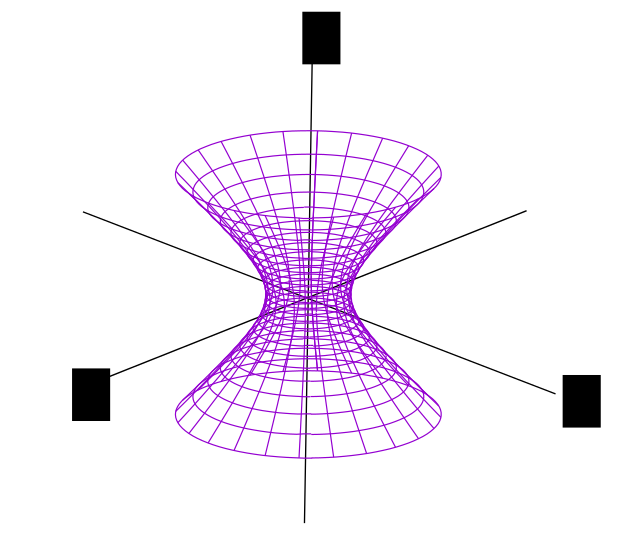
\includegraphics[width=0.49\textwidth]{images/onesheet}
	&
	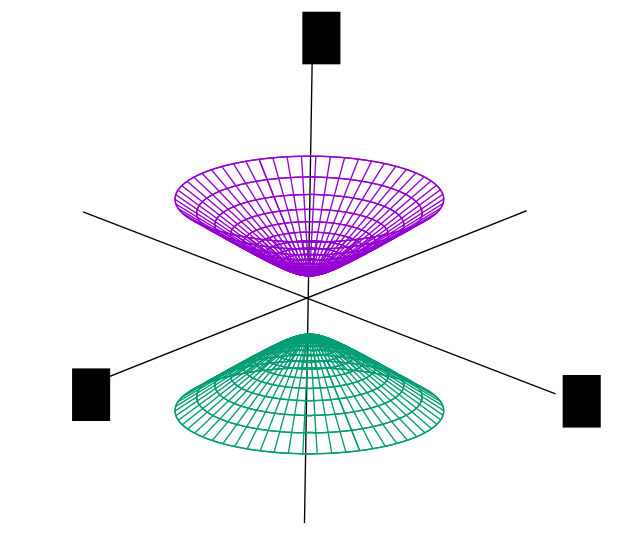
\includegraphics[width=0.49\textwidth]{images/twosheet}\\

	A Hyperboloid of one sheet 
	&
	A Hyperboloid of two sheet\\\\
\end{tabular}
\footnote{Svg files of these figures in the /image source. Please, look at this file}

\par
a, b, c are semi-axes and 0 the center of the surface. They are of revolution when a=b.

Similar surfaces are obtained for other combinations of signs.

The equations

\begin{align*}
	\frac{(x-h)^2}{a^2} + \frac{(y-k)^2}{b^2} - \frac{(z-l)^2}{c^2} = 1, \qquad -\frac{(x-h)^2}{a^2} - \frac{(y-k)^2}{b^2} + \frac{(z-l)^2}{c^2} = 1
\end{align*}

\noindent represent clearly hyperboloids with the same orientation of axes but center at (h, k, l).\\

\begin{hEnumerateAlpha} 
	\item Consider the equations \footnote{Please, look at prev. page. This is "c)"}
\end{hEnumerateAlpha}
 
\begin{align*}
	\frac{x^2}{a^2} + \frac{y^2}{b^2} = \lambda z \quad (EP), \qquad \frac{x^2}{a^2} - \frac{y^2}{b^2} = \lambda z \quad (HP)
\end{align*}

\end{document}
